\section{Research} \label{questions}
    In this section the research questions for the thesis are formulated. What is research method will be used and how the questions are being validated.

    \subsection{Context}
    What is the context of the research. 
    
   % Creation of test oracles are out of scope.
    
    % due to the experiment below sentence is false
    %The main research question will be around finding bugs with two inferred models. Even though generating models is needed, no research will be executed on generating those.
    
    %We can also test the outcome of TESTAR by infering models of the same version SUT and comparing those two models. Those two models should not contain any differences. 

    \subsection{Research questions}
        
        \textbf{Main research question is:} How can model diff help testers finding bugs???
        %% specify: "What form of the answer
        %% remove ambiguity
        %% specify: which factors influences the RQ
        
        %- What can TESTAR learn from Murphy?
        
        \begin{questions}
            \item Which code-changes can create a usable graph for difference \label{rq:model-changes}
            \item On which level do we need to find changes \label{rq:model-change-level}
        \end{questions}
        
        Since Murphy discovered difference with the help of Image comparison
        
        
        \begin{questions}[resume]
            \item Which classification can be given to a difference in two state diagrams? \label{rq:classifications} 
            \begin{questions}
                \item Which algorithm can be used to find differences between two state diagrams? \label{rq:algorithm}    
            \end{questions}
        \end{questions}
        
        The current algorithm \cite{stateDiff} makes two classifications regarding differences in state-diagrams; added and removed state. As a consequence, two state changes are observed when an action in the \acrshort{sut} is moved. For instance, an about window is moved from the \verb|File| to the \verb|Help| menu. 
        
        The hypothesis of \ref{rq:classifications} is that it can help the tester understand what kind of change is made to a new version of the \acrshort{sut}. In addition to the classification of differences, an investigation is needed on how to find differences (\ref{rq:algorithm}).
        
        %Image recognition might help in telling difference.
        %Could it be possible to use abstract image recognition. make a screenshot of an SUT and then fill in parts, like a Text box as a rectangle, button as a solid block etc. 
        % 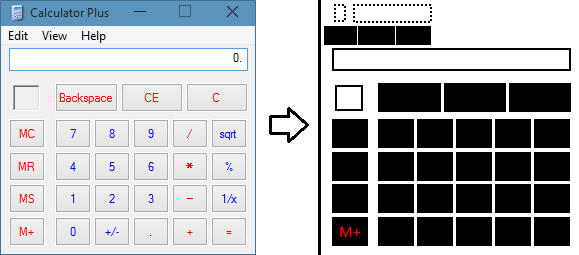
\includegraphics{document/pics/abstract-ui.png}
        
        \begin{questions}[resume]
            \item What tooling is available to show differences between two or more given state diagrams? \label{rq:differenceTool}
        \end{questions}
        
        With \ref{rq:differenceTool} we also need to include the current state model viewer \cite{thesisMulders}
        
        %- How can difference in the state model become visible inside build-in state model visualisation?
        
        %- How does the build-in state model work?
        
        %sub question: How to get a useful model for the model diff.
        %what is a useful model... -> depends on model diff requirements
        
        %sub question- How can we tell TESTAR to ignore complete entire widgets for state abstraction?
    

    \subsection{Research method}
    
        A literature study will be conducted for \ref{rq:algorithm} and \ref{rq:differenceTool}. 
        
        % add starting papers for each research question.
        
    \subsection{Validity}
    
        The answer to \ref{rq:algorithm} can keep changing -> important is to determine what kind of algorithm is good enough to be used in TESTAR.
        
        A thread to conclusion of \ref{rq:differenceTool} can be that researches or companies are trying to sell a product -> therefor write material which favors their product -> With all material assessing the objectivity of the material is of great importance. -> Might need to express the favor of the current viewer \cite{thesisMulders} but that could downgrade the conclusion of \ref{rq:differenceTool}. 
        
        Before refactoring, unit tests needs to be made -> can only  make unit test based on current implementation with the assumption that all units are working correctly as is. -> We can verify this by comparing the generated state model before and after refactoring.